\section{Data} \label{sec:data}
\subsection{NASA-Sloan Atlas}  \label{sec:nsa}
For our observations, we use galaxy photometry from the NASA-Sloan
Atlas\footnote{\url{http://www.nsatlas.org/}} (hereafter NSA).
The NSA provides photometry of $z < 0.05$ galaxies observed by the Sloan
Digital Sky Survey Data Release 8~\citep[SDSS;][]{aihara2011} with
improved background subtraction~\citep{blanton2011}. 
In particular, we use optical $g$, $r$, $i$, $z$ band absoluate magnitudes
derived using {\sc kcorrect}~\citep{blanton2007}, assuming a
\cite{chabrier2003} initial mass function. 
In Fig.~\ref{fig:nsa}, we present the $(g - r) - M_r$ color-magnitude
distribution of $\sim120,000$ NSA galaxies (black), which reveals the modes 
that correspond to blue star-forming and red quiescent galaxies. 

Among the full NSA sample, we focus on luminous galaxies with 
$-18 > M_r > -22$.
We exclude galaxies brighter than $M_r > -22$ since our simulated galaxy sample
does not include a large number of the most luminous galaxies. 
In addition, we only select galaxies with precisely measured photometry: 
magnitude uncertainties below $\sigma_g, \sigma_r, \sigma_i < 0.022$ and 
$\sigma_z < 0.04$. 
Lastly, we impose the color cuts to exclude galaxies within the
central 68 percentile of the $g-r$, $g-i$, $g-z$, $r-i$, $r-z$, $i-z$ color
distributions.
The color cuts remove NSA galaxies that potentially have observational
artifacts or problematic photometry.
They also ensure that the NSA galaxies are within the photometric distribution
(\ie~support) of the simulated galaxies used in this work.
We mark the 95$^{th}$ percentile contour of our NSA subsample in
Fig.~\ref{fig:nsa} (black dot-dashed).
In total, we use 14,736 NSA galaxies.


\begin{figure}[ht]
\vskip 0.2in
\begin{center}
    \centerline{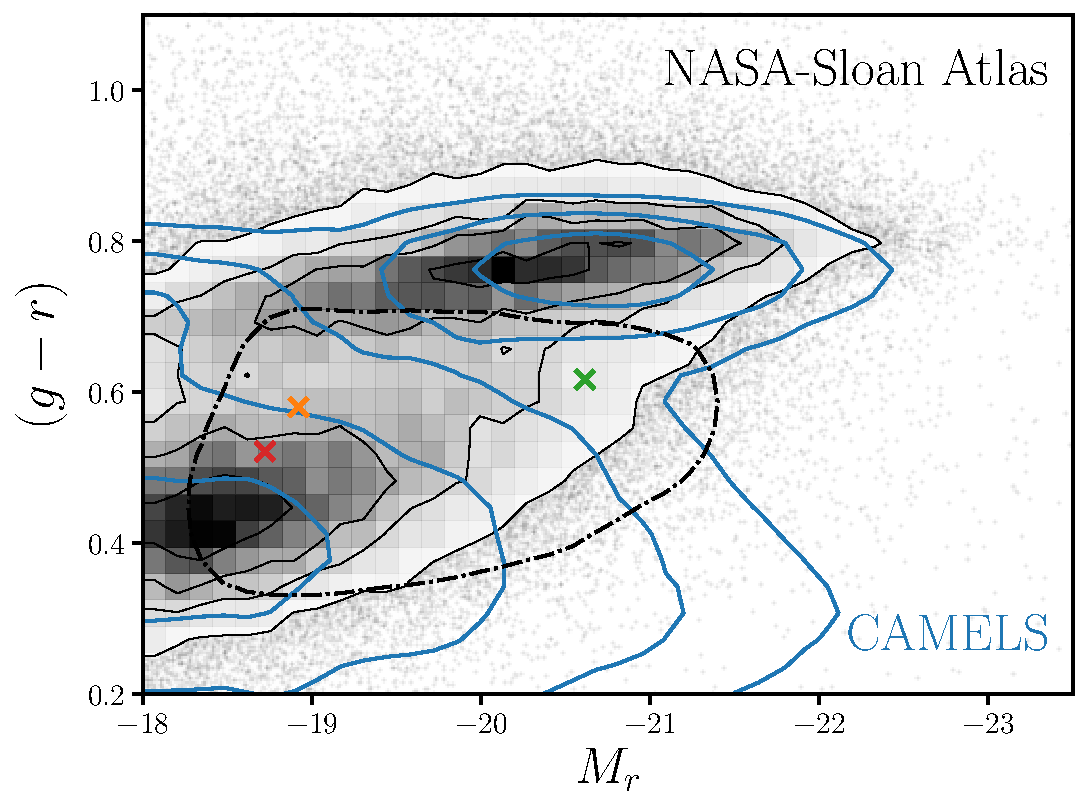
\includegraphics[width=\columnwidth]{figs/nsa.pdf}}
    \caption{Color-magnitude distrubtion, $(g-r) - M_r$, of observed galaxies
    from the NSA (black) and simulated galaxies from CAMELS-TNG (blue). 
    The distribution reveals the bimodality distribution of blue star-forming
    and red quiescent galaxies. 
    Overall, the distributions of NSA and CAMELS-TNG galaxies are in good
    agreement. 
    The distribution for CAMELS-TNG is significantly broader since its simulated
    galaxies are generated using a wide range of cosmological and baryonic
    feedback parameters.
    }\label{fig:nsa}
\end{center}
\vskip -0.2in
\end{figure}

\subsection{Forward Model: CAMELS} \label{sec:sims} 
In this work, we also use simulated galaxies from the Cosmology and
Astrophysics with MachinE Learning
Simulations~\citep[CAMELS;]{villaescusa-navarro2021, villaescusa-navarro2022a},
a suite of hydrodynamical simulations constructed over a wide
range of cosmological and hydrodynamical parameters.
In particular, we use the 1,000 hydrodynamical simulations (CAMELS-TNG)
constructed using the subrid physics model of the state-of-the-art
IllustrisTNG~\citep{nelson2019}. 
The simulations are generated with different cosmoloigcal parameters,
$\Omega = \{\Omega_m, \sigma_8\}$, and baryonic feedback parameters, 
$\mathcal{B} = \{A_{\rm SN1}, A_{\rm SN2}, A_{\rm AGN1}, A_{\rm AGN2}\}$,
arranged in a latin hypercube. 
$A_{\rm SN1}$ and $A_{\rm SN2}$ represent the normalization factors for the 
galactic wind flux and speed; 
$A_{\rm AGN1}$ and $A_{\rm AGN2}$ represent the normalization factors for the 
energy output and specific energy of AGN feedback.

The CAMELS-TNG simulation all have a comoving volume of 
(25 $h^{-1}{\rm Mpc}$)$^3$.
They each evolve $256^3$ dark matter particles and $256^3$ fluid elements from
$z=127$ to $z=0$ from initial conditions generated using second order
perturbation theory. 
Each simulation has 34 saved snapshots from $z=6$ to $z=0$. 
Since we target $z < 0.05$ NSA galaxies, we only use the $z=0$ snapshot. 
All the cosmological parameter besides $\Omega_m$ and $\sigma_8$ are fixed:
$\Omega_b = 0.049$, $h = 0.6711$, $n_s = 0.9624$, $\sum m_\nu = 0.0$eV, and 
$w = -1$.
The SUBFIND~\citep{springel2001, dolag2009} algorithm is run on each simulation
to identify halos and subhalos.
SUBFIND computes physical quantities of the subhalos and the galaxies that
resides in them. 
For additional details on CAMELS, we refer readers to
\cite{villaescusa-navarro2021, villaescusa-navarro2022a}.

In all 1,000 CAMELS-TNG simulations, there are $\sim$700,000 galaxies with more
than 20 star particles. 
The galaxies, however, are not evenly distributed across the simulations and
have a significant dependence on the CAMELS parameters.  
For instance, simulations constructed at higher $\Omega_m$ values have more
galaxies.  
Since the goal of this work is to conduct cosmological inference on a per
galaxy basis, we must correct for this implicit prior on the CAMELS parameters.
We do this by randomly selecting 100 galaxies from each simulation. 
This imposes a uniform prior: $p(\Omega, \mathcal{B}) = 1$. 
Thus, we use a total of 100,000 CAMELS-TNG galaxies.  

Since the goal of this work is to analyze the observed photometry of NSA
galaxies, we forward model observed photometry for the simulated galaxies. 
CAMELS-TNG already provides synthetic dust attenuated stellar photometry for
each simulated galaxy calculated using the same procedure as \cite{nelson2018}.
The unattenuated spectral energy distribution (SED) of a galaxy is computed by
combining the SEDs of every member star particle of the host subhalo. 
Each star particle SED is modeled as a single-burst simple stellar population
using stellar population synthesis (SPS) based on the recorded birth time,
metallicity, and mass. 
The SPS uses FSPS~\citep{conroy2009, conroy2010}, Padova isochrones, MILES
stellar library, and assumes a Chabrier initial mass function. 
The unattenuated galaxy SEDs are then dust attenuated using the ``Model C'' dust
model of \cite{nelson2018}, which is based on the metal content of the neutral
gas distribution in and around each galaxy. 
Afterwards, each galaxy SED is convolved with the SDSS $g$, $r$, $i$, $z$-band
photometric bandpasses to produce the photometry: $X_i$. 
For additional details on the synthetic photometry, we refer readers to
\cite{nelson2018}. 

The synthetic photometry in CAMELS-TNG does not include any uncertainties.
However, since we have measured uncertainties, $\sigma_X$, for NSA galaxies, we
can construct a realistic noise model. 
For each CAMELS-TNG galaxy, we randomly sample $\sigma_{X,i}$ from the range of
uncertainties measured in NSA. 
Afterwards, we apply the uncertainty using a Gaussian with standard deviation
$\sigma_{X,i}$: $\hat{X}_i \sim \mathcal{N}(X_i, \sigma_{X, i})$. 
Our noise model does not include correlations between the magnitudes and the
uncertainties. 
However, as we later discuss, this is not an issue in our approach beacuse the
posteriors we ultimately evaluate are conditioned on the uncertainties. 
In Fig.~\ref{fig:nsa}, we present the color-magnitude distribution of the
forward modeled CAMELS-TNG galaxies in blue. 
